\documentclass[11pt]{article}
\usepackage[a4paper,margin=0.86in]{geometry}
\usepackage{amsmath,amssymb,bm,mathtools}
\usepackage{booktabs,longtable,tabularx,array}
\usepackage{tikz}
\usetikzlibrary{positioning,arrows.meta,fit}
\usepackage{microtype}
\usepackage{hyperref}
\usepackage{enumitem}
\usepackage{setspace}
\hypersetup{colorlinks=true,linkcolor=black,citecolor=black,urlcolor=blue}
\setstretch{1.05}
\newcommand{\R}{\mathbb{R}}
\newcommand{\Prob}{\mathcal P}
\newcommand{\E}{\mathbb E}
\newcommand{\Id}{\mathrm{id}}
\newcommand{\TV}{\mathrm{TV}}
\newcommand{\KL}{D_{\mathrm{KL}}}
\title{\textbf{Functorial Epigenetic Realignment (FER):\\ Reversing Topological Drift via Information-Geometric Optimal Transport and Mechanotransductive Acoustic Holography}}
\author{Devanik Debnath (Devanik21)\\\small Department of Electronics and Communication Engineering, National Institute of Technology Agartala, India\\\small ORCID: 0009-0001-8310-6921}
\date{8 October 2026}
\begin{document}
\maketitle

\begin{center}
\fbox{\begin{minipage}{0.90\textwidth}
\textbf{Research posture.} This paper is a theoretical and computational proposal. It does not establish that aging is caused by topology alone, that a youthful topological state is unique, that ultrasound can restore chromatin, or that any human treatment is safe or effective. The mathematical contribution is an explicit composition of topological descriptors, information geometry, optimal transport, constrained control, mechanobiology, and acoustic field synthesis into a falsifiable research program.
\end{minipage}}
\end{center}

\begin{abstract}
Aging is a multiscale process involving molecular, cellular, tissue, and systemic interactions. A central problem is therefore how to represent an age-associated cellular state without reducing it to one biomarker or one pathway. We introduce \emph{Functorial Epigenetic Realignment} (FER), a geometric-control framework in which a cellular population is represented simultaneously by a probability distribution over a learned multi-omic feature space and by a multiscale topological signature of regulatory, chromatin, and nuclear organization. FER defines an information-geometric state manifold, a Wasserstein transport geometry between age-defined reference states, an identity-preserving optimal-control problem, and a category-theoretic consistency condition for mapping abstract state transitions into admissible physical controls. Mechanotransduction through the cytoskeleton, LINC complex, nuclear lamina, and chromatin is treated as a candidate coupling, while acoustic holography is treated as a candidate field-synthesis interface for controlled \emph{in vitro} experiments.

The paper separates five epistemic levels: exact mathematical identities (P1), variational and dynamical selection (P2), statistical universality (P3), cross-domain structural mappings (P4), and visual analogy (P5). The key proposal is not that aging is ``really geometry.'' Rather, it is that a geometric representation might supply a measurable target space for state control. The framework produces explicit falsification criteria: topological reproducibility across held-out donors, alignment between observed trajectories and the predicted transport direction, preservation of lineage identity and genomic integrity, and a calibrated relationship between mechanical observables and state displacement. A deterministic NumPy verification script establishes the corresponding toy mathematical identities, including exact H1 computation on a clique complex, one-dimensional Wasserstein geodesics, Fisher-Rao geometry, minimum-norm linearized control, functorial composition, Lindblad trace preservation, and paired nematic defect charge neutrality. None of these computations constitute biological or clinical evidence.
\end{abstract}

\section{Problem statement}
The dominant quantitative descriptions of aging are mechanistic and molecular. Current frameworks emphasize multiple interacting processes rather than one root cause \cite{lopezotin2023}. Epigenetic drift, chromatin reorganization, cellular senescence, inflammation, metabolic change, and tissue-level mechanical remodeling can all coexist. The practical consequence is that two cells may have similar measurements along one molecular axis while differing strongly in regulatory relations, nuclear architecture, or mechanical state.

FER asks whether these heterogeneous measurements admit a useful state-space geometry. The target is not an abstract philosophical claim. A useful geometric representation should satisfy four operational requirements:
\begin{enumerate}[leftmargin=1.45em]
\item it should compress high-dimensional observations without destroying experimentally meaningful structure;
\item it should define distances between age-associated states that are stable under resampling and batch variation;
\item it should identify a target direction that can be compared against measured trajectories after perturbation; and
\item it should include explicit penalties for lineage loss, genomic damage, and mechanically pathological responses.
\end{enumerate}

The ``crumpled paper'' analogy motivates the question but is not a proof. Cells are chemical, physical, and dynamical systems. Nuclear geometry is one layer of their state, not a replacement for chemistry.

\section{Literature position and scope of novelty}
Recent work makes the individual ingredients of FER scientifically relevant. The aging literature explicitly includes epigenetic alterations among interconnected hallmarks \cite{lopezotin2023}. Reviews of reprogramming-induced rejuvenation emphasize both the reversibility of some age-associated epigenetic states and the requirement to preserve cell identity \cite{gama2018,yucel2024,li2026}. Three-dimensional chromatin organization is increasingly measured as an age- and senescence-associated variable, including changes in compartments, topologically associating domains, and enhancer-promoter interactions \cite{sun2018,ma2026}.

Topological data analysis has already been proposed as a framework for studying aging and extracting multiscale signatures from complex biological data \cite{fulop2020}. Optimal transport is an established mathematical tool for reconstructing cellular trajectories, including developmental and reprogramming trajectories from single-cell data \cite{schiebinger2019}. Mechanobiology has established mechanical coupling between extracellular and cytoskeletal structures, the nuclear envelope, and chromatin organization \cite{miroshnikova2017,lityagina2021,miroshnikova2022,kloc2025}. At the same time, mechanical stress can cause DNA damage and pathological epigenetic memory, which makes a damage-aware controller essential rather than optional \cite{qiu2025,boyle2026}.

Active-matter theory provides rigorous mathematics for defects in ordered biological systems, but current results do not establish that a senescent cell is a topological defect in the strict sense \cite{marchetti2013,angheluta2026,beer2026}. Acoustic holography can synthesize shaped ultrasound fields, and recent work has begun to demonstrate spatially selective fields in cultured-cell experiments; neither result demonstrates subcellular epigenome control in intact human tissue \cite{burstow2025,fujita2026}.

Accordingly, the novelty claim of FER is deliberately operational. The paper defines a specific composition of established mathematical and physical modules with an experimentally measurable objective and pre-specified failure conditions. A finite literature search cannot prove that no equivalent idea has ever been conceived globally. The scientific contribution is instead the reproducible specification of the proposed architecture.

\section{Epistemic hierarchy}
The framework follows five levels to prevent cross-domain category errors.
\begin{longtable}{p{0.10\textwidth}p{0.31\textwidth}p{0.51\textwidth}}
\toprule
Level & Meaning & Use in FER \\
\midrule
P1 & Algebraic or topological identity & Betti-number identities, Wasserstein definitions, Fisher metric, functor composition, trace preservation, defect winding. \\
P2 & Dynamical or variational selection & Minimum-action transport and constrained control. \\
P3 & Statistical or universality claim & Cross-donor, cross-batch, and cross-scale stability of learned signatures. \\
P4 & Cross-domain structural mapping & Mapping state-space directions to mechanically realized control directions. \\
P5 & Visual analogy & The crumpled-paper intuition; it is explanatory only. \\
\bottomrule
\end{longtable}

\begin{figure}[t]
\centering
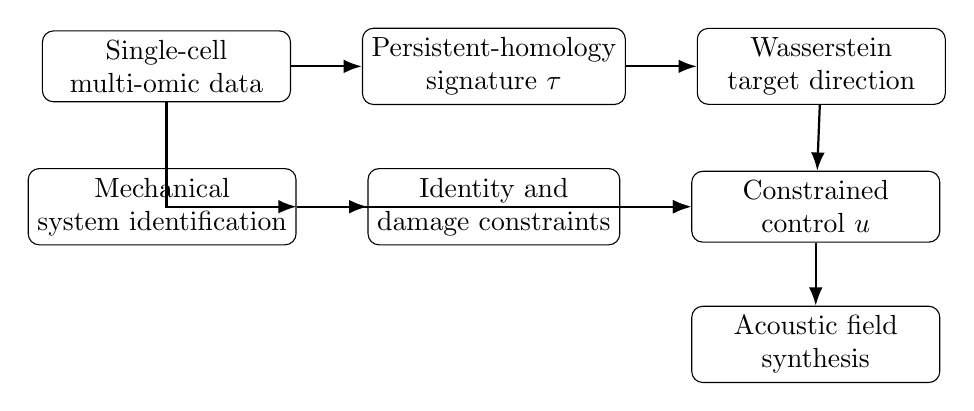
\begin{tikzpicture}[
  node distance=8mm and 9mm,
  box/.style={draw,rounded corners,align=center,minimum width=3.15cm,minimum height=9mm},
  arrow/.style={-Latex,thick}
]
\node[box] (data) {Single-cell\\multi-omic data};
\node[box,right=of data] (top) {Persistent-homology\\signature $\tau$};
\node[box,right=of top] (ot) {Wasserstein\\target direction};
\node[box,below=of top] (id) {Identity and\\damage constraints};
\node[box,left=of id] (mech) {Mechanical\\system identification};
\node[box,right=of id] (ctrl) {Constrained\\control $u$};
\node[box,below=of ctrl] (field) {Acoustic field\\synthesis};
\draw[arrow] (data) -- (top);
\draw[arrow] (data) |- (mech);
\draw[arrow] (top) -- (ot);
\draw[arrow] (ot) -- (ctrl);
\draw[arrow] (id) -- (ctrl);
\draw[arrow] (mech) -- (id);
\draw[arrow] (mech) -- (ctrl);
\draw[arrow] (ctrl) -- (field);
\end{tikzpicture}
\caption{FER research stack. The topological and transport representations define a target direction, while identity and damage constraints restrict admissible state motion. Mechanical transfer functions are identified experimentally before acoustic field synthesis is attempted.}
\label{fig:ferstack}
\end{figure}

\section{State representation}
Let a standardized cell observation be
\begin{equation}
 x = \left(x_{\mathrm{RNA}},x_{\mathrm{ATAC}},x_{\mathrm{meth}},x_{\mathrm{hist}},x_{\mathrm{prot}},x_{\mathrm{3D}},x_{\mathrm{nuc}}\right) \in \R^d.
\label{eq:x}
\end{equation}
Here the components denote transcriptomic, chromatin-accessibility, methylation, histone, proteomic, three-dimensional genomic, and nuclear-mechanical measurements. Not every experiment must contain every modality. The state space is learned from an explicitly specified feature map so that preprocessing decisions are part of the model and are not hidden.

A cell population is represented by a probability measure $p \in \Prob(\mathcal X)$ rather than by a single centroid. Let $p_y$ denote a reference distribution estimated from a young cell population and $p_a$ an aged distribution. Crucially, these distributions are conditioned on cell identity and experimental context; a bulk distribution that mixes cell types can otherwise manufacture apparent rejuvenation by changing composition.

\section{Information geometry}
On the interior of the probability simplex, a natural local metric is the Fisher information metric
\begin{equation}
 g_p(u,v)=\sum_{i=1}^{d}\frac{u_i v_i}{p_i},
\label{eq:fisher}
\end{equation}
for tangent vectors satisfying the simplex constraint. The corresponding norm is
\begin{equation}
 \|u\|_{g_p}^2 = g_p(u,u).
\label{eq:fishernorm}
\end{equation}
This metric penalizes displacement in low-probability coordinates more strongly than an unweighted Euclidean metric. In FER it serves as a local geometry for state sensitivity; it is not asserted to be the unique biological metric.

An information-theoretic admissibility bound follows from Pinsker's inequality:
\begin{equation}
 \TV(p,q) \leq \sqrt{\frac{1}{2}\KL(p\|q)}.
\label{eq:pinsker}
\end{equation}
The bound is useful as a conservative relation between an information divergence and total-variation state discrepancy. It does not convert information distance into a biological age score.

\section{Topological state descriptors}
Suppose a feature map embeds cells into a metric space and a filtration $K_\epsilon$ is built, for example through a Vietoris-Rips construction. Persistent homology returns persistence diagrams $D_k$. The associated Betti curve is
\begin{equation}
 \beta_k(\epsilon)=\mathrm{rank}\,H_k(K_\epsilon).
\label{eq:betti}
\end{equation}
A topological signature can therefore be written as
\begin{equation}
 \tau = \left\{\beta_0(K_\epsilon),\beta_1(K_\epsilon),\ldots,\beta_K(K_\epsilon)\right\}_{\epsilon\in\mathcal E}.
\label{eq:tau}
\end{equation}
In practice, the persistence diagrams can also be converted to persistence landscapes or persistence images for statistical learning. The stability of persistence diagrams under perturbations supports the use of such descriptors, but stability does not imply causality \cite{cohensteiner2007}.

We define a generic topological discrepancy by
\begin{equation}
 d_{\mathrm{top}}^2(\tau_1,\tau_2)=\sum_{k=0}^{K}\omega_k \|\Phi(D_k^{(1)})-\Phi(D_k^{(2)})\|_2^2,
\label{eq:topdist}
\end{equation}
where $\Phi$ is a fixed vectorization map and $\omega_k\geq 0$ are pre-registered weights. The weights must be fixed on a training set and evaluated on a held-out set to avoid leakage.

A critical restriction follows. A large change in $d_{\mathrm{top}}$ is not automatically a biological aging event. The topological descriptor becomes scientifically useful only when it predicts held-out functional or molecular outcomes beyond appropriate null models.

\section{Optimal transport as a target geometry}
The quadratic Wasserstein distance between discrete distributions is
\begin{equation}
 W_2^2(p_a,p_y)=\min_{\pi\in\Pi(p_a,p_y)}\sum_{i,j} c_{ij}\pi_{ij},
\label{eq:w2}
\end{equation}
where $\Pi(p_a,p_y)$ preserves the marginals and $c_{ij}$ is a ground cost. The ground metric is not innocuous: a Euclidean cost after arbitrary feature scaling can create an artificial geometry. FER therefore requires that the feature normalization, ground metric, and modality weights be reported and stress-tested.

In the continuous setting, the Benamou-Brenier dynamic formulation is
\begin{equation}
 W_2^2(\rho_0,\rho_1)=\inf_{\rho,v}\int_0^1\int_{\mathcal X}\rho_t(x)\|v_t(x)\|^2\,dx\,dt,
\label{eq:bb}
\end{equation}
subject to the continuity equation
\begin{equation}
 \partial_t\rho_t+\nabla\cdot(\rho_t v_t)=0.
\label{eq:continuity}
\end{equation}
Thus the transport geodesic is a minimum kinetic-action interpolation in the chosen geometry.

For one-dimensional distributions, let $Q_0$ and $Q_1$ denote quantile functions. The constant-speed path is
\begin{equation}
 Q_t=(1-t)Q_0+tQ_1.
\label{eq:quantile}
\end{equation}
It satisfies
\begin{equation}
 W_2(p_s,p_t)=|t-s|W_2(p_0,p_1),
\label{eq:constant}
\end{equation}
under the standard one-dimensional construction. The numerical verification script tests this identity on a deterministic toy distribution.

\section{Composite target functional}
FER combines the geometries and biological constraints through
\begin{equation}
 \mathcal D(z,z_y)=\alpha W_2^2(p_z,p_y)+\beta d_{\mathrm{top}}^2(\tau_z,\tau_y)+\gamma R_{\mathrm{id}}(z,z_0)+\lambda R_{\mathrm{stress}}(z),
\label{eq:composite}
\end{equation}
where $z_0$ is the initial state, $R_{\mathrm{id}}$ quantifies lineage-identity departure, and $R_{\mathrm{stress}}$ penalizes mechanically unsafe or genomically damaging states.

One possible identity penalty is
\begin{equation}
 R_{\mathrm{id}}(z,z_0)=\|h_{\mathrm{lineage}}(z)-h_{\mathrm{lineage}}(z_0)\|_2^2,
\label{eq:idpenalty}
\end{equation}
with $h_{\mathrm{lineage}}$ a pre-registered lineage representation. The exact choice is an empirical question.

A stress penalty may be a weighted functional over measured nuclear strain, DNA-damage markers, cell-cycle state, and pathological mechanosignaling:
\begin{equation}
 R_{\mathrm{stress}}(z)=\sum_r \kappa_r\,\psi_r(m_r(z)),
\label{eq:stresspenalty}
\end{equation}
where each $\psi_r$ is zero inside an admissible region and increases outside it.

\section{Constrained state dynamics}
Let $z(t)$ denote the latent biological state and $u(t)$ the abstract actuator coordinate. The local controlled dynamics are
\begin{equation}
 \dot z=f(z)+G(z)u+\eta,
\label{eq:dynamics}
\end{equation}
where $f$ is endogenous drift, $G$ is the calibrated input-response operator, and $\eta$ collects unmodeled variation and measurement noise.

The optimal-control objective is
\begin{equation}
 \mathcal J[u]=\int_0^T\left[\frac{1}{2}\|u(t)\|_{R}^2+\alpha W_2^2(p_{z(t)},p_y)+\beta d_{\mathrm{top}}^2(\tau_{z(t)},\tau_y)+\gamma R_{\mathrm{id}}+\lambda R_{\mathrm{stress}}\right]dt,
\label{eq:controlobjective}
\end{equation}
subject to Eq.~\eqref{eq:dynamics} and control bounds $u(t)\in\mathcal U$.

The interpretation is deliberately conservative. The controller seeks low-cost, admissible motion toward a target distribution; it does not infer a biological law from the existence of a mathematical geodesic.

\section{A local minimum-norm control proposition}
Consider a local linearization $\dot z=A u$ for a desired tangent $v$. When $A$ has full row rank, the Moore-Penrose solution
\begin{equation}
 u^*=A^\dagger v
\label{eq:pseudoinverse}
\end{equation}
is the unique minimum-Euclidean-norm solution of $Au=v$.

\paragraph{Proof sketch.} Every solution can be written as $u=A^\dagger v+n$ with $n$ in the null space of $A$. The minimum-norm pseudoinverse solution is orthogonal to that null space. Therefore
\begin{equation}
 \|u\|_2^2=\|A^\dagger v\|_2^2+\|n\|_2^2\geq\|A^\dagger v\|_2^2.
\label{eq:minnorm}
\end{equation}
The verification script checks both the reconstruction residual and the null-space orthogonality condition on a toy full-rank matrix.

\section{Functorial translation}
Define a category $\mathsf E$ whose objects are admissible biological states $(z,\tau,p,h)$ and whose morphisms are admissible state trajectories or transition operators. Define a category $\mathsf A$ whose objects are physically realizable control states and whose morphisms are calibrated actuator transformations.

The FER translation is a functor
\begin{equation}
 F:\mathsf E\rightarrow\mathsf A.
\label{eq:functor}
\end{equation}
Functoriality requires
\begin{equation}
 F(\Id_z)=\Id_{F(z)}
\label{eq:functorid}
\end{equation}
and
\begin{equation}
 F(g\circ f)=F(g)\circ F(f).
\label{eq:functorcomp}
\end{equation}

The practical meaning is that a sequence of experimentally composable biological transitions should map to a correspondingly composable sequence of actuator transformations. If two state transitions are not independently identifiable, no categorical notation can repair that missing calibration.

\section{Differential-geometric coupling to mechanics}
Let $\xi(\mathbf r,t)$ denote displacement and $\varepsilon=\frac12(\nabla\xi+\nabla\xi^\top)$ the infinitesimal strain tensor. A generic linearized viscoelastic continuum satisfies
\begin{equation}
 \rho_m\,\partial_t^2\xi=\nabla\cdot\sigma(\varepsilon,\dot\varepsilon,z)+b,
\label{eq:continuum}
\end{equation}
with constitutive law
\begin{equation}
 \sigma=C(z):\varepsilon+D(z):\dot\varepsilon.
\label{eq:constitutive}
\end{equation}
The dependence of $C$ and $D$ on latent state $z$ is a measurable hypothesis rather than an assumed constant.

A coarse nuclear coupling can be represented as a traction transfer
\begin{equation}
 t_n=K_L(\xi_c-\xi_n),
\label{eq:linc}
\end{equation}
where $\xi_c$ and $\xi_n$ are cytoskeletal and nuclear displacements and $K_L$ is an effective coupling tensor. Eq.~\eqref{eq:linc} is a phenomenological abstraction of force transmission through the cytoskeleton, LINC complex, and nuclear lamina. It does not identify a particular chromatin locus as a direct acoustic target.

\section{Active matter and defect variables}
Ordered multicellular systems can exhibit polar or nematic patterns with localized defects. Active-matter theory provides a well-defined language for these defects and their dynamics \cite{marchetti2013,angheluta2026,beer2026}. FER proposes a restricted P4 hypothesis: tissue-scale order parameters may improve state description and may provide a useful coarse variable for mechanical control.

There is no basis here for the stronger statement that a senescent cell is literally a topological defect. To test such a claim, one would require a field variable, an order parameter, a defect core definition, and a reproducible association between defect charge or defect density and independently defined senescence phenotypes.

For a nematic director angle $\theta(\mathbf r)$, a closed-contour charge is
\begin{equation}
 q=\frac{1}{4\pi}\oint_C d(2\theta).
\label{eq:nematiccharge}
\end{equation}
A +1/2 and -1/2 pair therefore has net charge zero. This is a topological identity, not a rejuvenation mechanism.

\section{Acoustic field synthesis}
Acoustic holography is capable of spatially shaping ultrasound fields through phase and amplitude control \cite{burstow2025,fujita2026}. In abstract form,
\begin{equation}
 p(\mathbf r,t)=\mathrm{Re}\left\{\sum_{m=1}^{M}a_m(\mathbf r)e^{i(\mathbf k_m\cdot\mathbf r-\omega_m t+\phi_m)}\right\}.
\label{eq:acoustic}
\end{equation}
The inverse field-design problem can be represented as
\begin{equation}
 J_{\mathrm{field}}(u)=\|\mathcal H u-p^*\|_2^2+\lambda_u\|u\|_2^2,
\label{eq:fieldobjective}
\end{equation}
where $\mathcal H$ is an experimentally calibrated acoustic forward operator.

The major conceptual boundary is spatial scale. A field can be focused or shaped at an imaging-relevant or cellular scale without implying that a specific chromatin domain has been deterministically displaced. The required transfer function from external acoustic field to nuclear/chromatin state is unknown. It must therefore be measured.

\section{Open-system operator formulation}
For completeness, a finite-dimensional latent coarse-graining can be represented by a positive operator $\varrho(t)$ with an open-system generator
\begin{equation}
 \dot\varrho=-i[H(z),\varrho]+\sum_k\left(L_k\varrho L_k^\dagger-\frac12\{L_k^\dagger L_k,\varrho\}\right).
\label{eq:lindblad}
\end{equation}
This is used only as a mathematical bookkeeping device for noisy, dissipative latent states. FER does not claim biologically coherent quantum dynamics at therapeutic length scales. The numerical check verifies trace preservation of a simple toy dissipator.

A useful tensor-network representation can similarly factorize a high-order multi-omic tensor $X$ as a tensor train:
\begin{equation}
 X_{i_1\ldots i_n}\approx\sum_{r_0,\ldots,r_n}G^{(1)}_{r_0i_1r_1}G^{(2)}_{r_1i_2r_2}\cdots G^{(n)}_{r_{n-1}i_nr_n},
\label{eq:tensortrain}
\end{equation}
with boundary ranks fixed to one. This is a computational factorization, not a statement that a cell is a quantum tensor network.

\section{FER control algorithm}
The full algorithm can be written as a sequence of measurable transformations:
\begin{enumerate}[leftmargin=1.45em]
\item \textbf{Reference construction:} estimate $p_y$, $\tau_y$, and identity representation $h_y$ from donor-balanced reference cells.
\item \textbf{Topology extraction:} build a pre-registered filtration and calculate persistence summaries.
\item \textbf{Geometric target:} compute the transport geometry from $p_a$ to $p_y$.
\item \textbf{Constraint assembly:} define lineage, proliferation, genomic-integrity, and stress admissibility regions.
\item \textbf{System identification:} estimate $G(z)$ from perturbation-response experiments.
\item \textbf{Control synthesis:} solve Eq.~\eqref{eq:controlobjective} under measured constraints.
\item \textbf{Field realization:} if acoustic forcing is used, solve Eq.~\eqref{eq:fieldobjective} against a calibrated mechanical observable rather than directly against a presumed chromatin state.
\item \textbf{Outcome test:} measure the resulting state trajectory at single-cell resolution and compare it with the predicted target direction.
\end{enumerate}

This ordering is important. It prevents the inverse problem from becoming a speculative frequency-search exercise before the biological transfer function is known.

\section{Experimental design and statistical discipline}
\subsection{Data structure}
The first studies should use donor-matched cultured cells with independently defined young and aged conditions. Single-cell sampling is required so that apparent rejuvenation is not caused by selective survival or population composition shifts.

\subsection{Null models}
At minimum, analysis should include:
\begin{enumerate}[leftmargin=1.45em]
\item feature-shuffle nulls that preserve marginal distributions;
\item degree-preserving graph nulls when graph topology is used;
\item donor-block label permutations;
\item batch-only models;
\item cell-cycle and proliferation covariates; and
\item composition-matched comparisons.
\end{enumerate}

\subsection{Cross-validation}
All topological embeddings, metric weights, feature transformations, and controller parameters must be learned on training donors and frozen before validation. Test donors must be held out from model-selection decisions.

\subsection{Primary alignment statistic}
Let $v_{\mathrm{OT}}$ be the target tangent predicted by the transport model and $v_{\mathrm{obs}}$ the measured state velocity. Define
\begin{equation}
 A_{\mathrm{OT}}=\frac{\langle v_{\mathrm{obs}},v_{\mathrm{OT}}\rangle}{\|v_{\mathrm{obs}}\|\,\|v_{\mathrm{OT}}\|}.
\label{eq:alignment}
\end{equation}
The value is meaningful only relative to donor-blocked and permutation-based null distributions. A controller that merely changes the magnitude of a generic state coordinate without directional agreement does not support the FER hypothesis.

\subsection{Identity constraint}
A successful experiment must jointly report age-associated state movement and identity preservation. Suggested readouts include lineage markers, transcriptomic identity classifiers, proliferation, karyotype or genomic-integrity assays where appropriate, DNA-damage markers, and cell function.

\section{Falsification criteria}
FER contains multiple nested hypotheses.
\begin{enumerate}[leftmargin=1.45em]
\item \textbf{H1: topological representation.} A learned topological signature predicts age-defined state or function in held-out donors beyond null models.
\item \textbf{H2: geometric direction.} Perturbations that improve a pre-registered functional endpoint show directional agreement with the target-state transport geometry.
\item \textbf{H3: mechanical coupling.} A calibrated mechanical observable predicts state displacement after conditioning on energy and exposure duration.
\item \textbf{H4: controllability.} The estimated local map $G(z)$ has sufficient rank and stability that an admissible control can move the state in a target direction without violating stress and identity constraints.
\item \textbf{H5: field realization.} A shaped external field can reproduce the required mechanical observable within the experimentally admissible range.
\end{enumerate}

Failure of any necessary link rejects the corresponding level of the model. In particular, H5 can fail even if H1-H4 succeed, because a biologically useful mechanical trajectory may not be externally realizable with ultrasound.

\section{Safety constraints}
Mechanical forcing is not inherently rejuvenating. The same mechanotransduction pathways that permit adaptive responses can create pathological state changes. Recent experimental work links mechanical stress, Piezo1 signaling, Rho-ROCK activity, histone modification, and persistent disease-associated mechanical memory in cancer models \cite{boyle2026}. Reviews of nuclear mechanics also emphasize that excessive deformation can damage the genome \cite{qiu2025,kloc2025}.

FER therefore defines safety as a constrained optimization problem. An admissible controller must satisfy
\begin{equation}
 R_{\mathrm{stress}}(z(t))\leq \delta_{\mathrm{stress}},
\qquad
 R_{\mathrm{id}}(z(t),z_0)\leq \delta_{\mathrm{id}},
\label{eq:constraints}
\end{equation}
for all relevant $t$, with thresholds determined experimentally and pre-registered for each model system.

No human treatment parameters are specified in this paper.

\section{Relation to molecular reprogramming}
The FER framework should be viewed as a potential additional control layer rather than a replacement for molecular approaches. Partial reprogramming is being actively studied as a means of resetting aspects of cellular age while attempting to preserve cell identity \cite{yucel2024,li2026}. First-in-human testing of a cellular rejuvenation approach has entered clinical development in 2026, but such work does not by itself establish whole-body lifespan extension \cite{naturebiotech2026}.

The critical comparison is therefore experimental. If mechanical control produces no unique predictive value after controlling for molecular perturbation, FER adds little. If mechanical variables improve control efficiency, specificity, or identity preservation, they may constitute a useful orthogonal intervention dimension.

\section{Predictions}
The strongest predictions are quantitative.
\begin{enumerate}[leftmargin=1.45em]
\item Age-defined donor cohorts will contain reproducible multiscale topological differences after controlling for sequencing depth, cell type, and batch.
\item Some mechanically perturbed trajectories will occupy directions closer to the transport geodesic than matched energy controls.
\item Mechanical observables will explain a measurable fraction of state displacement after accounting for exposure magnitude.
\item Controllers constrained by identity and damage metrics will outperform unconstrained controllers on multi-objective score, even if they move more slowly.
\item The relationship between external acoustic field and chromatin-state displacement will be substantially tissue- and cell-state-dependent; a universal frequency-to-epigenome map is not expected.
\end{enumerate}

\section{Numerical verification}
The accompanying \texttt{verify\_model.py} script is intentionally small and deterministic. It does not claim to simulate biology. It establishes the internal consistency of the mathematical abstractions used by the manuscript.

First, a ring-like and a contractile-line point cloud are converted into radius graphs and then into clique complexes through dimension two. The script computes the exact $H_1$ Betti number over $\mathrm{GF}(2)$, using
\begin{equation}
 \beta_1=E-\mathrm{rank}(B_1)-\mathrm{rank}(B_2).
\label{eq:beta1complex}
\end{equation}
This is still a toy proxy for a biological topological filtration.

Second, two one-dimensional distributions are transported by quantile interpolation. The program checks constant step speed and the exact $t^2W_2^2$ displacement law.

Third, a full-rank linearized control map is inverted with the Moore-Penrose pseudoinverse, and the solution's null-space orthogonality is tested.

Fourth, functorial composition and identity are checked in a deliberately linear toy category.

Fifth, a two-level Lindblad dissipator is tested for trace preservation, solely as an operator-mechanics identity.

Sixth, nematic defect charges are computed exactly on a closed contour and verified to sum to zero for a paired +1/2 and -1/2 construction.

The code output is a reproducibility certificate for the equations, not a biological result.

\section{Limitations}
\begin{enumerate}[leftmargin=1.45em]
\item \textbf{Topology is representation-dependent.} The filtration, metric, sampling density, and feature scaling affect the observed persistence structure.
\item \textbf{Optimal transport is not biology.} A geodesic minimizes a mathematical action in a chosen geometry; biological systems may be unable to realize it.
\item \textbf{Functoriality is not causality.} A structure-preserving map cannot substitute for an experimentally identified transfer function.
\item \textbf{Mechanotransduction is context-dependent.} Cell type, extracellular matrix, cytoskeletal state, nuclear stiffness, and signaling state can reverse or modify responses.
\item \textbf{Defects are a hypothesis at the aging level.} Active-matter defect mathematics is established, but a strict defect interpretation of senescence remains untested.
\item \textbf{Acoustic penetration is not epigenome addressability.} Shaping a field in tissue does not imply deterministic control over nuclear chromatin domains.
\item \textbf{Systemic aging is outside the current model.} Immune, endocrine, vascular, metabolic, neural, and whole-organism feedback are not represented explicitly.
\end{enumerate}

\section{Research program and decision gates}
The work should advance only when each gate is satisfied.
\begin{longtable}{p{0.13\textwidth}p{0.30\textwidth}p{0.48\textwidth}}
\toprule
Gate & Question & Advancement criterion \\
\midrule
G1 & Is the topological signature reproducible? & Held-out donor performance exceeds pre-registered nulls. \\
G2 & Does transport direction predict useful state motion? & Directional agreement exceeds blocked-label nulls. \\
G3 & Is mechanical coupling identifiable? & $G(z)$ is stable over perturbation replicates and predicts state response. \\
G4 & Can control be constrained? & Target motion is achieved without violating identity/damage limits. \\
G5 & Can an external field reproduce the required mechanics? & Calibrated field-to-mechanics fidelity passes a pre-registered threshold. \\
G6 & Does the intervention improve biology? & Functional benefit survives independent replication and safety analysis. \\
\bottomrule
\end{longtable}

A failure at G1-G5 should stop progression to more complex models rather than trigger stronger forcing or broader claims.

\section{Conclusion}
FER proposes a geometric-control formulation of an aging-state problem. The central hypothesis is not that aging is reducible to topology, but that biological state may contain a predictive geometric layer that is useful for control.

The framework connects persistent homology, information geometry, Wasserstein transport, categorical composition, mechanotransduction, active-matter variables, and acoustic field synthesis. The novelty is expressed as a falsifiable architecture rather than a claim of metaphysical priority or proof of global conceptual novelty.

The scientifically meaningful outcome is therefore straightforward. If topology provides a robust state signature, if transport geometry predicts experimentally observed improvement directions, and if mechanical perturbations can reproducibly control those directions without damaging identity or genomic integrity, then geometry has become a practical control variable in aging biology. If these links fail, the framework should be rejected or narrowed accordingly.

\section*{Data and Code Availability}
The release contains \texttt{verify\_model.py}, which uses Python 3 and NumPy only. No external dataset is required to reproduce the mathematical checks. Biological validation is intentionally deferred to future, regulated experimental work.

\section*{Author digital research footprint}
GitHub: \url{https://github.com/Devanik21/The-Invention-Archive}\\
Medium: \url{https://medium.com/@devanik2005}\\
X: \url{https://x.com/devanik2005}\\
LinkedIn: \url{https://www.linkedin.com/in/devanik}\\
ORCID: \url{https://orcid.org/0009-0001-8310-6921}\\
Kaggle: \url{https://www.kaggle.com/devanikdebnath}

Zenodo, OpenAIRE, and Google Scholar are discovery/indexing destinations only after a persistent record actually exists. No record or indexing status is inferred from this metadata file.

\bibliographystyle{plain}
\bibliography{paper}
\end{document}